\section{Auswertung}
\label{sec:Auswertung}
Sämtliche im Folgenden durchgeführten Ausgleichsrechnungen werden mit der \emph{curve fit} Funktion aus dem für \emph{Python} geschriebenen package \emph{NumPy}\cite{scipy} durchgeführt. Fehlerrechnungen werden mit dem für \emph{Python} geschriebenen package \emph{Uncertainties}\cite{uncertainties} ausgeführt.

\subsection{Stehende Schallwellen in einer Röhre}
\label{sec:Ausw1}
Zunächst wird ein Übersichtsspektrum einer $\SI{60}{\centi\meter}$ langen Röhre, bestehend aus acht je $\SI{75}{\milli\meter}$ langen Teilstücken, aufgenommen, siehe Abbildung \ref{fig:1_1}.
\begin{figure}
  \centering
  \includegraphics{build/1_overview.pdf}
  \caption{Übersichtsspektrum einer 8$\times\SI{75}{\milli\meter}$ Röhre.}
  \label{fig:1_1}
\end{figure}
Nun wird das Spektrum einer $\SI{15}{\centi\meter}$ langen Röhre, bestehend aus zwei je $\SI{75}{\milli\meter}$ langen Teilstücken, aufgenommen und näher untersucht. Hierzu muss die Dämpfung auf einen geeigneten Wert eingestellt werden. Dazu sind Spektren mit verschiedenen Dämpfungseinstellungen verglichen worden. Mit abnehmender Dämpfung macht sich dabei der Effekt bemerkbar, dass die größten Amplituden aus Spektren größerer Dämpfung immer weiter abgeschnitten werden. Dies ist ein Anzeichen für nicht-lineares Verhalten des Systems. Der Wert der Dämpfung wird so eingestellt, dass das System noch im linearen Bereich arbeitet und somit die aufgenommenen Amplituden tatsächlich proportional zu den Amplituden der untersuchten Schallwelle sind.

Für die Analyse des Spektrums wird die Fit-Funktion des Programms SpectrumSLC\cite{skript} verwendet. Der resultierende Fit ist zusammen mit den Messwerten in Abbildung \ref{fig:1_2} dargestellt.
\begin{figure}
  \centering
  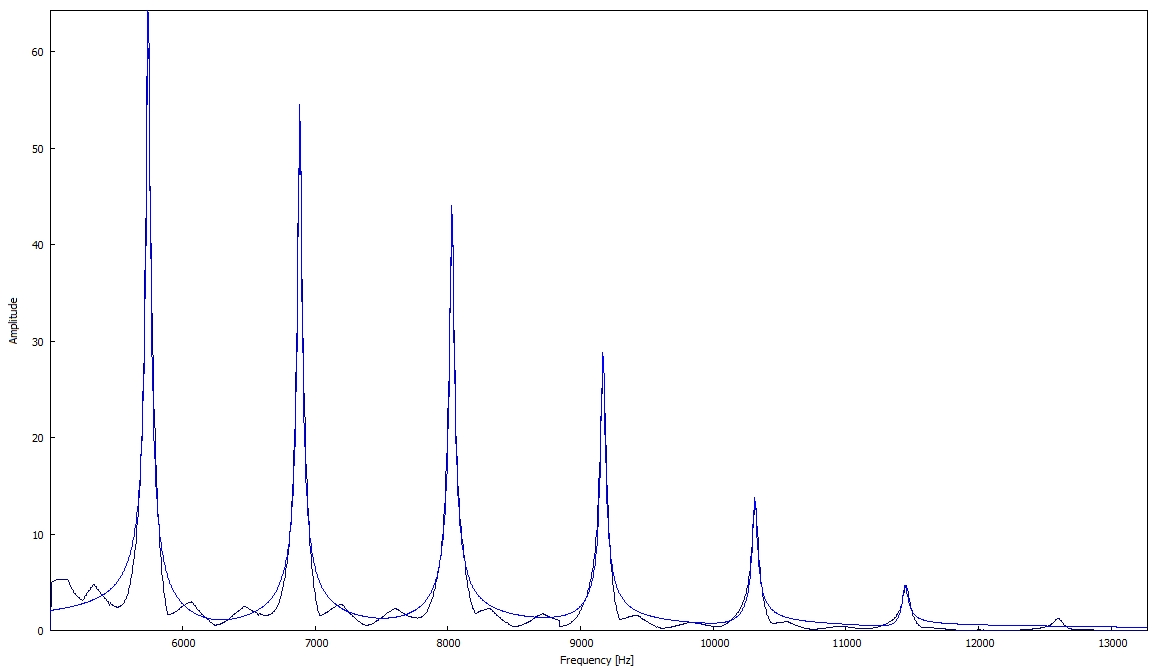
\includegraphics[width=0.8\textwidth]{messdaten/1--2Fit.jpg}
  \caption{Messdaten einer 2$\times\SI{75}{\milli\meter}$ Röhre und Fit (in blau) des Programms SpectrumSLC.}
  \label{fig:1_2}
\end{figure}
Die gefundenen Fitparameter sind für zwei durchgeführte Fits in den Tabellen \ref{table:1_2_fit1} und \ref{table:1_2_fit2} aufgeführt.
\input{build/1_2_fit1.tex}
\input{build/1_2_fit2.tex}
Es ist zu  erkennen, dass insbesondere der siebte Peak aufgrund der vergleichsweise geringen Amplitude durch beide Fits nicht korrekt wiedergegeben wird. Dies liegt an der Methode der Least-Squares. Ferner unterscheiden sich die restlichen Parameter aus den beiden Tabellen nur geringfügig. Generell sind die Peaks weiter rechts anfälliger für Ungenauigkeiten aufgrund des ungünstigeren Verhältnisses Amplitudenhöhe zu Peakbreite.
Es ist wie erwartet (siehe Gleichungen \eqref{eq:Breite} und \eqref{eq:omega}) eine Tendenz zu größeren Peakbreiten mit zunehmender Frequenz zu beobachten.

\subsection{Stehende Schallwellen in einem Kugelresonator}
\subsubsection{Vergleich des Spektrums bei verschiedenen Winkeln}
Es werden in 30° Abständen bezüglich des Winkels $\alpha$ der oberen Hemisphäre Spektren im Frequenzbereich 100 bis $\SI{10000}{\kilo\hertz}$ aufgenommen und in den folgenden Abbildungen \ref{fig:2_1} bis \ref{fig:2_7} dargestellt.
\begin{figure}
  \centering  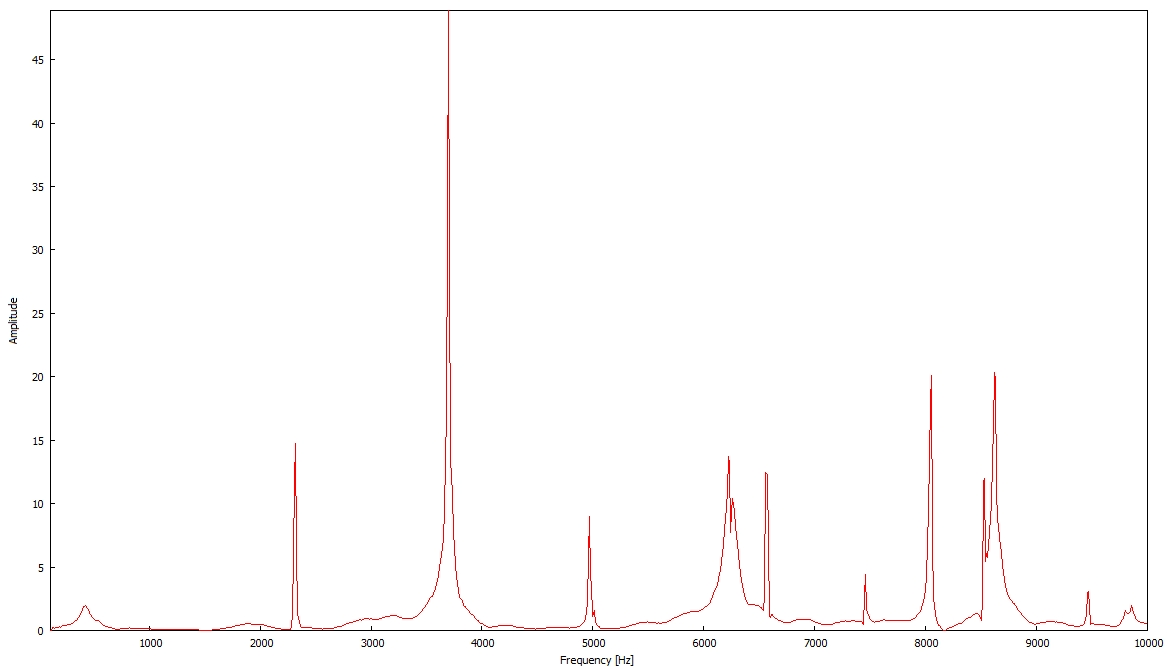
\includegraphics{build/2_1_00.pdf}  \caption{Spektrum bei $\alpha=0$°.} \label{fig:2_1}
\end{figure}
\begin{figure}
  \centering  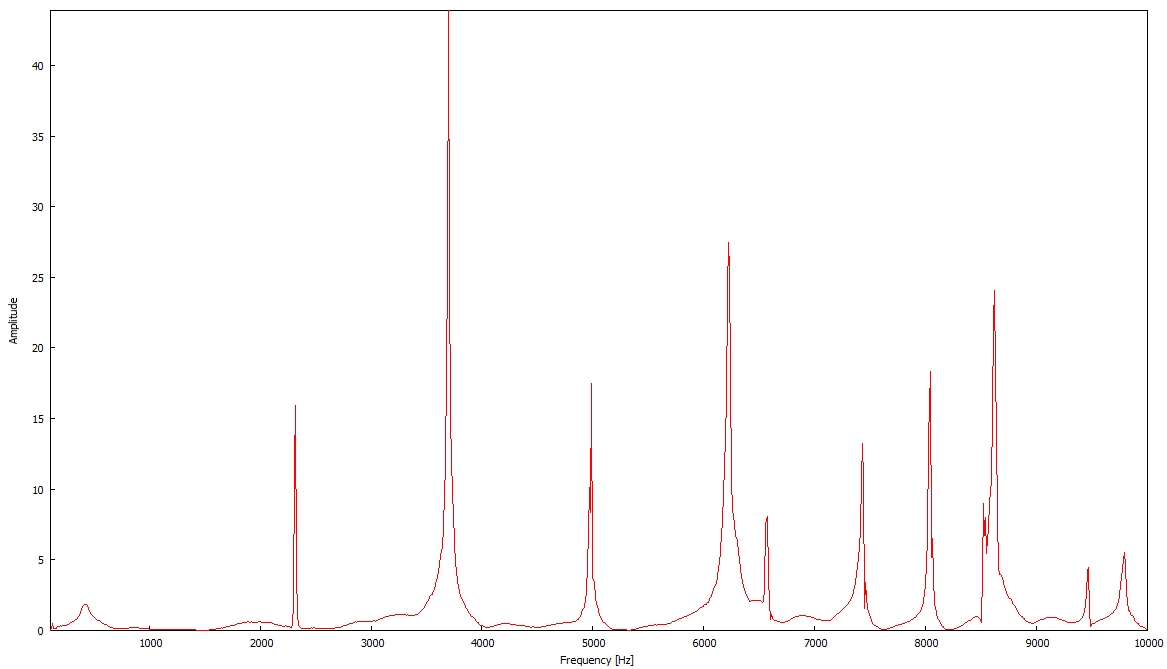
\includegraphics{build/2_1_30.pdf}  \caption{Spektrum bei $\alpha=30$°.} \label{fig:2_2}
\end{figure}
\begin{figure}
  \centering  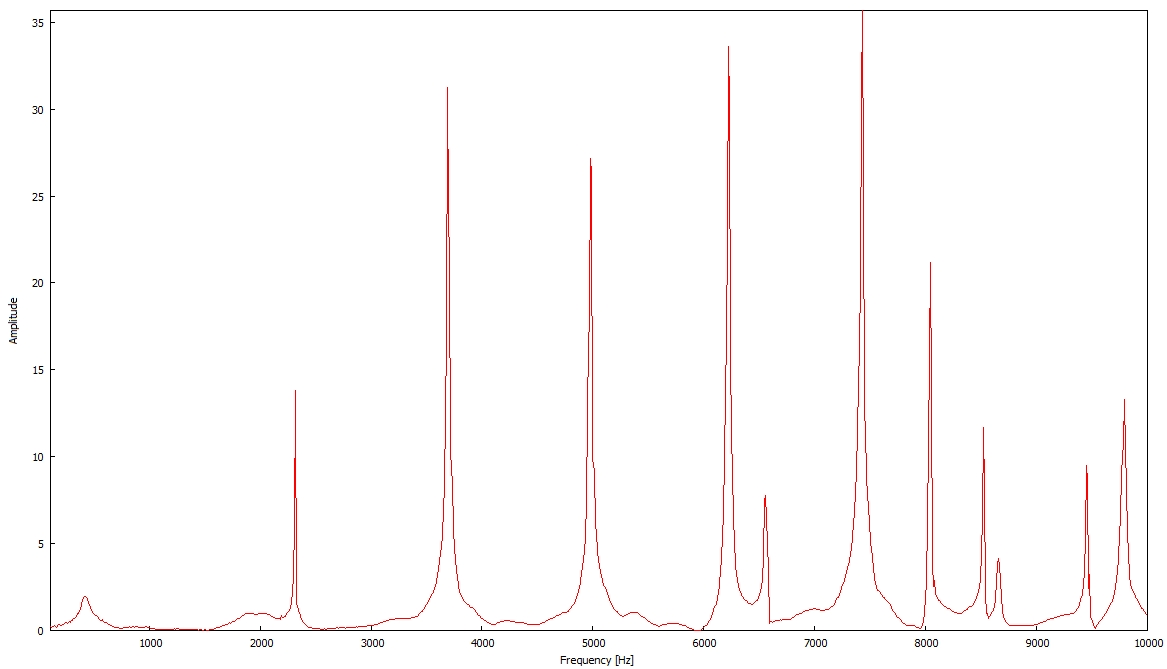
\includegraphics{build/2_1_60.pdf}  \caption{Spektrum bei $\alpha=60$°.} \label{fig:2_3}
\end{figure}
\begin{figure}
  \centering  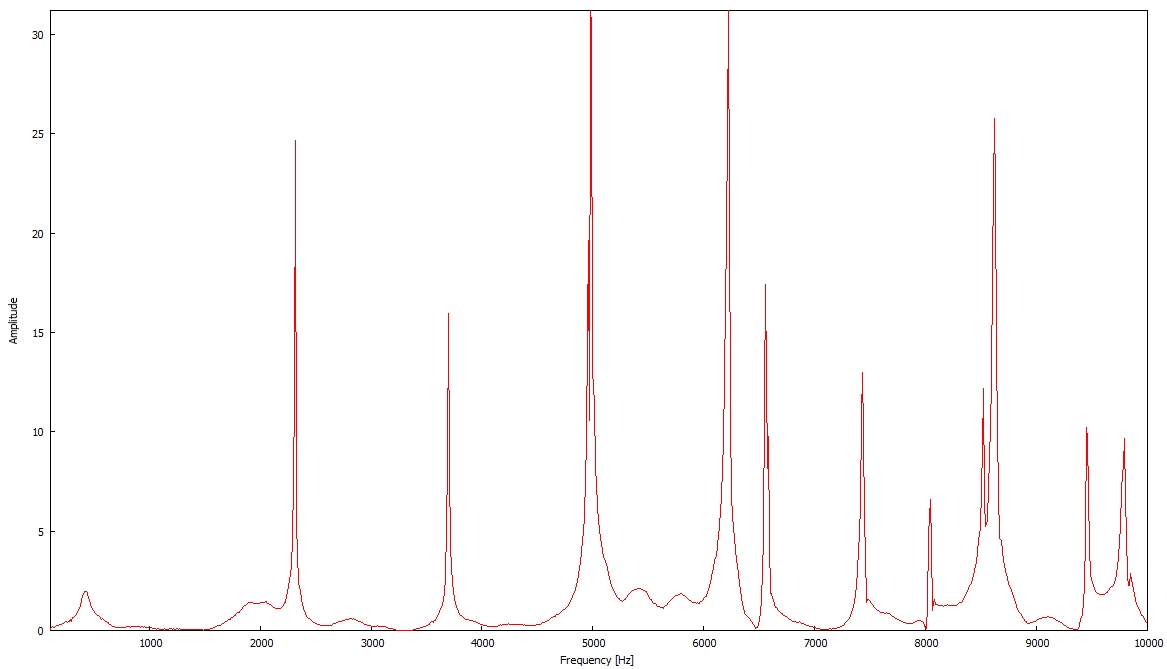
\includegraphics{build/2_1_90.pdf}  \caption{Spektrum bei $\alpha=90$°.} \label{fig:2_4}
\end{figure}
\begin{figure}
  \centering  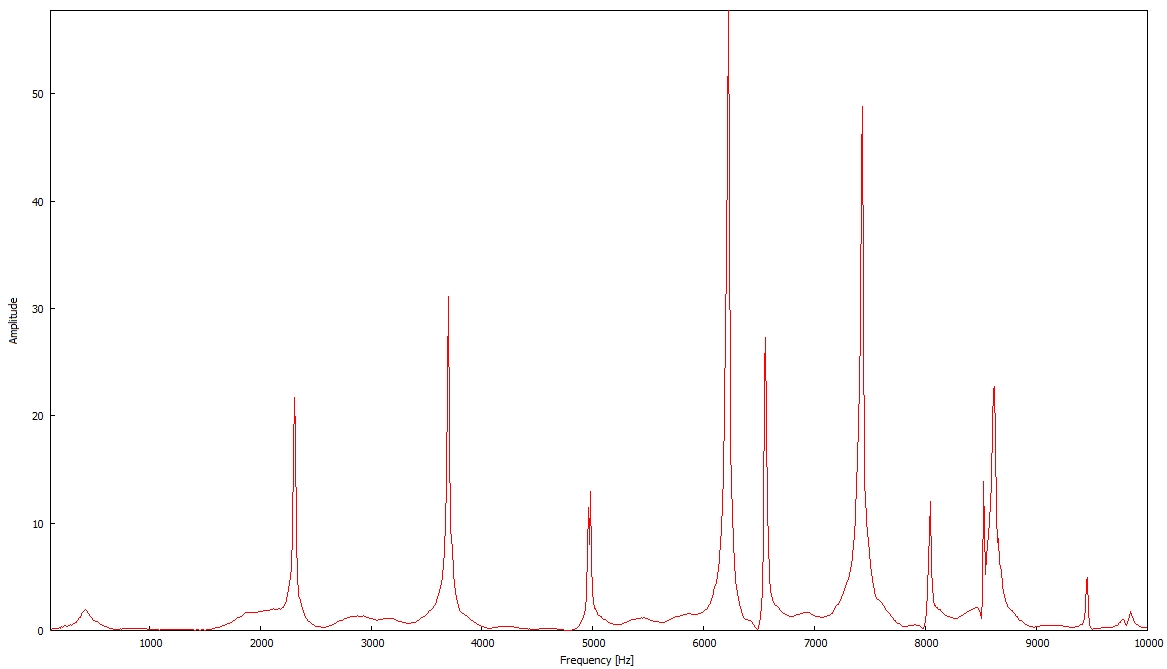
\includegraphics{build/2_1_120.pdf}  \caption{Spektrum bei $\alpha=120$°.} \label{fig:2_5}
\end{figure}
\begin{figure}
  \centering  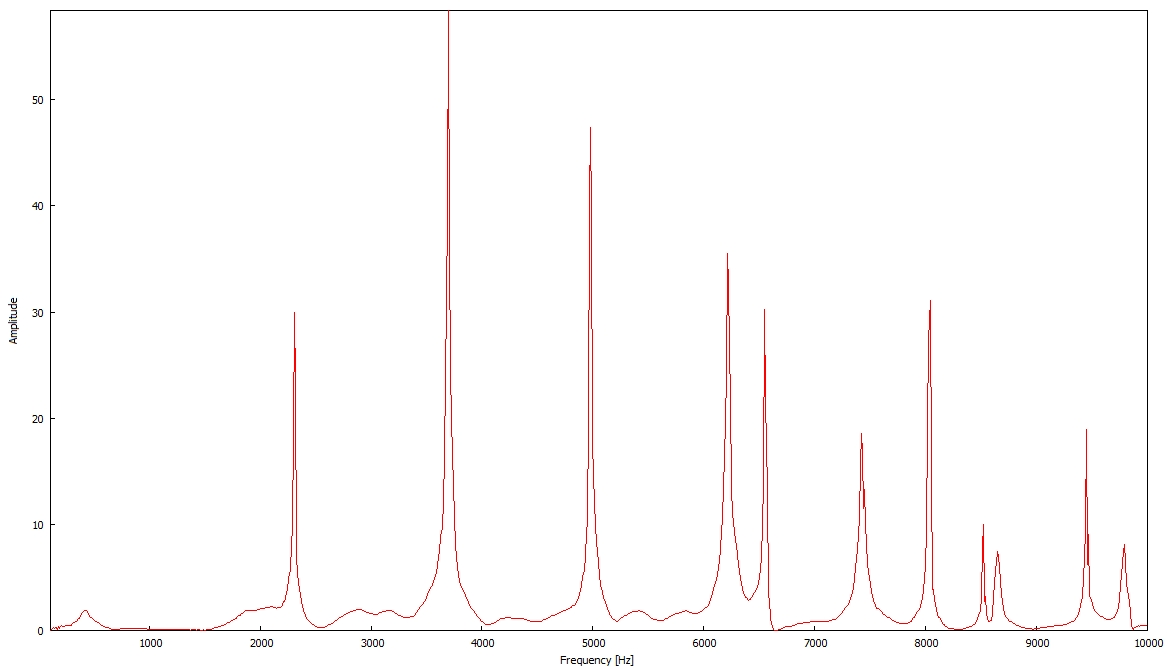
\includegraphics{build/2_1_150.pdf}  \caption{Spektrum bei $\alpha=150$°.} \label{fig:2_6}
\end{figure}
\begin{figure}
  \centering  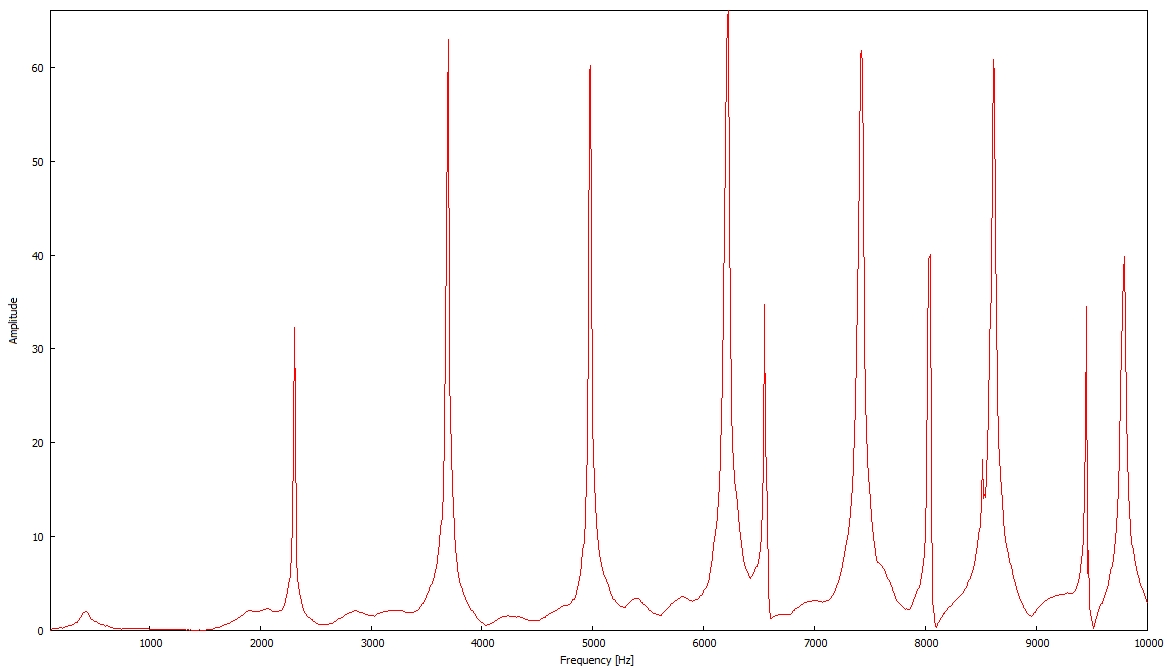
\includegraphics{build/2_1_180.pdf}  \caption{Spektrum bei $\alpha=180$°.} \label{fig:2_7}
\end{figure}
Die Peaks variieren in ihrer Amplitude mit dem Winkel, nicht jedoch in ihrer Frequenz. Dieses Verhalten ist zu erwarten, denn es zeigt die Winkelabhängigkeit der Kugelflächenfunktionen (vgl. die Werte für die Knoten des Legendrepolynoms in Abbildung \ref{fig:Anh1}). So nimmt zum Beispiel der Peak bei ca. $\SI{7400}{\hertz}$ für 0°, 30° und 90° sehr geringe Amplitudenwerte an, während für 60°, 120° und 180° der Peak stark ausgeprägt ist. Eine bessere Auflösung der Winkelabhängigkeit erfolgt in Kapitel \ref{sec:VisYlm}. An dieser Stelle ist noch festzuhalten, dass die Amplitude im Allgemeinen für $\alpha=180$° die größten Werte annimmt. Hier ist der Polarwinkel $\Theta=90$°.

\subsubsection{Untersuchung eines Doppelpeaks}
Ein Frequenzbereich, der sich für die Untersuchung der Winkelabhängigkeit eignet, ist derjenige um $\SI{5000}{\hertz}$, denn hier liegt ein Doppelpeak vor. Dieser wird in einer feineren Auflösung von $\SI{1}{\hertz}$ ausgemessen für drei verschiedene Winkel $\alpha=$0°, 20°, 40°. Eine zusammengeführte Darstellung findet sich in Abbildung \ref{fig:2_8} wieder.
\begin{figure}
  \centering
  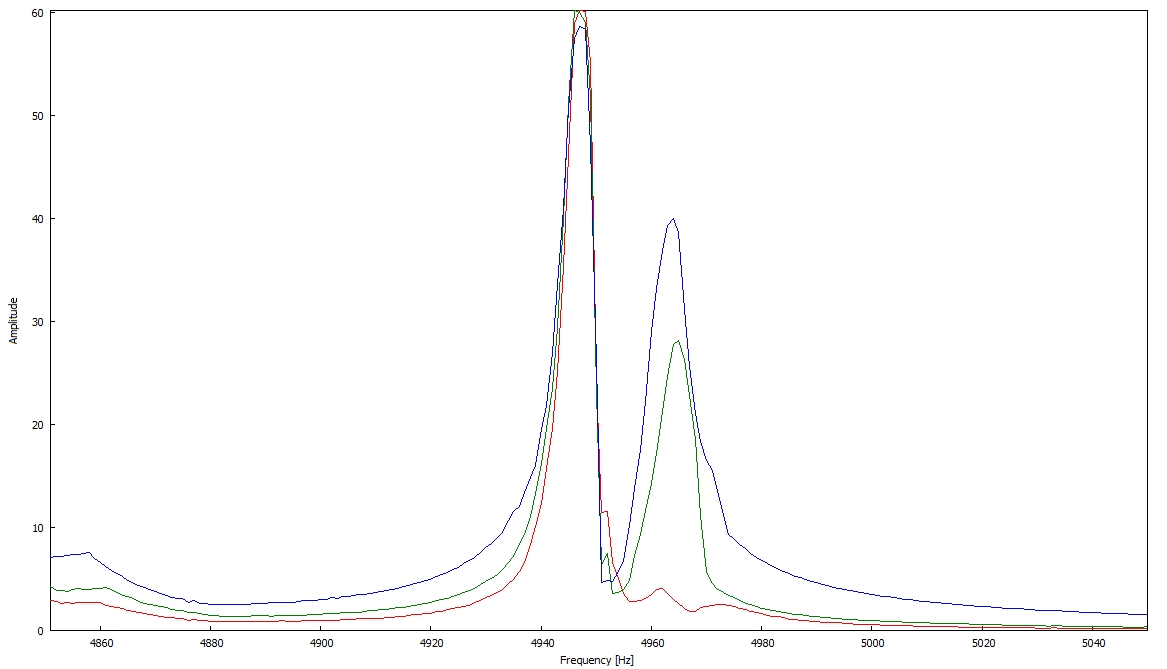
\includegraphics{build/2_2.pdf}  \caption{Doppelpeak bei verschiedenen Winkeln $\alpha$.} \label{fig:2_8}
\end{figure}
Es ist gut zu erkennen, dass der Peak bei $\SI{4960}{\hertz}$ für $\alpha=$0° nahezu verschwindet und erst mit größerem $\alpha$ sichtbar wird, während die Intensität des links davon liegenden Peaks unbeeinflusst bleibt.

\subsubsection{Visualisierung der Kugelflächenfunktionen}
\label{sec:VisYlm}
In diesem Abschnitt wird die Winkelauflösung für insgesamt fünf markante Peaks auf 10° verfeinert. So lässt sich für jeden Peak ein Polarplot erstellen, mit dessen Hilfe auf die Drehimpulsquantenzahl $l$ rückgeschlossen wird. Zunächst zeigt Abbildung \ref{fig:2_9} eine Übersicht bei $\alpha=$180° und in einem Frequenzbereich von 100 bis $\SI{7000}{\hertz}$.
\begin{figure}
  \centering
  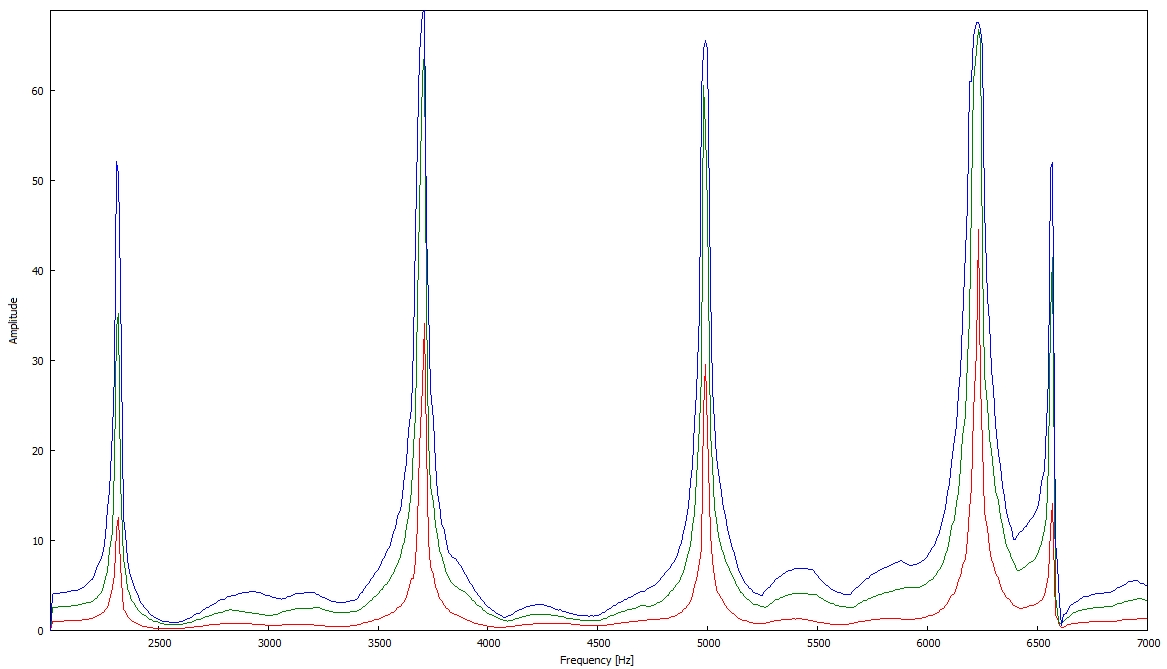
\includegraphics{build/2_3_overview.pdf}  \caption{Übersichtsspektrum bei $\alpha=$180°.} \label{fig:2_9}
\end{figure}
Hieraus werden die fünf erkennbaren Peaks ausgesucht und näher untersucht. Die Umrechnung des Winkels $\alpha$ in den Polarwinkel $\Theta$ geschieht gemäß Gleichung \eqref{eq:ThetaVonAlpha}. Während $\alpha$ zwar einen Bereich von 0° bis 180° abdeckt, kann $\Theta$ jedoch nur das Intervall 0° bis 90° durchlaufen. Die fehlenden Werte für 90° bis 180° werden durch eine Spiegelung symmetrisch aus den vorhandenen Daten erstellt. Somit ist also lediglich die Hälfte des sichtbaren Bereichs durch die Messung verifiziert. Schließlich wird durch eine erneute Spiegelung der Polarplot vervollständigt mit den -- mathematisch redundanten -- Werten 180° bis 360°. Die so entstehenden Polarplots sind in den Abbildungen \ref{fig:2_10} bis \ref{fig:2_14} dargestellt.
\begin{figure}
    \centering
    \begin{subfigure}[b]{0.475\textwidth}
        \centering
        \begin{minipage}{\textwidth}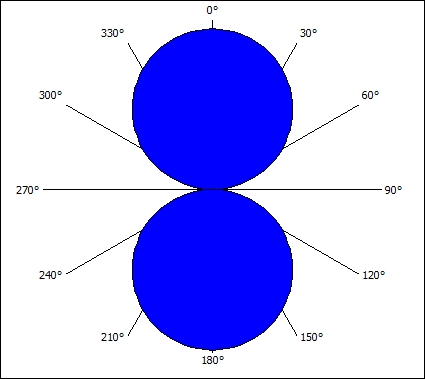
\includegraphics[width=\textwidth]{ressources/l1.jpg}\end{minipage}
        \caption[]%
        {{\small Theorie für $l=1$.}}
        \label{fig:2_10a}
    \end{subfigure}
    \hfill
    \begin{subfigure}[b]{0.475\textwidth}
        \centering
        \begin{minipage}{\textwidth}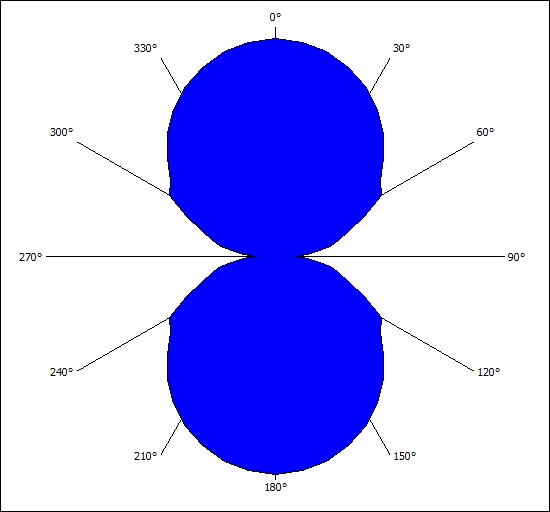
\includegraphics[width=\textwidth]{messdaten/2_3_2310.jpg}\end{minipage}
        \caption[]%
        {{\small Messung.}}
        \label{fig:2_10b}
    \end{subfigure}
    \caption[]
    {Polarplot für $f=\SI{2310}{\hertz}$.}
    \label{fig:2_10}
\end{figure}
\begin{figure}
    \centering
    \begin{subfigure}[b]{0.475\textwidth}
        \centering
        \begin{minipage}{\textwidth}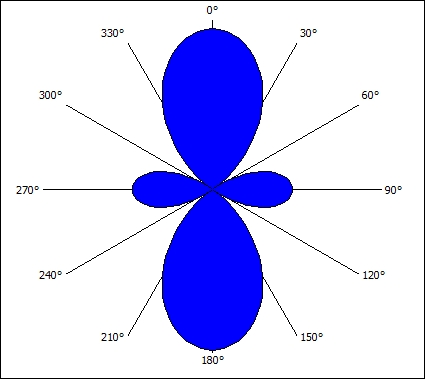
\includegraphics[width=\textwidth]{ressources/l2.jpg}\end{minipage}
        \caption[]%
        {{\small Theorie für $l=2$.}}
        \label{fig:2_11a}
    \end{subfigure}
    \hfill
    \begin{subfigure}[b]{0.475\textwidth}
        \centering
        \begin{minipage}{\textwidth}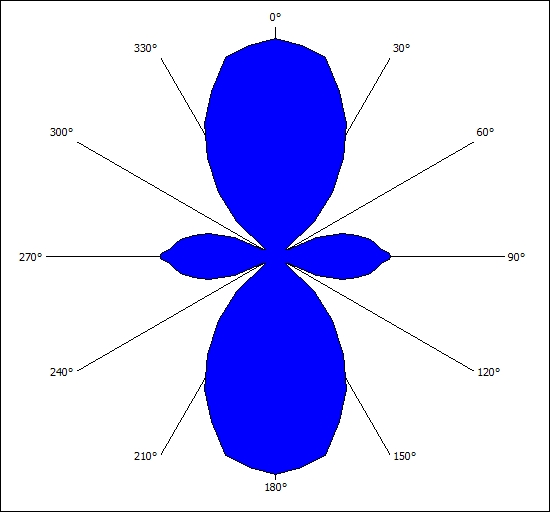
\includegraphics[width=\textwidth]{messdaten/2_3_3711.jpg}\end{minipage}
        \caption[]%
        {{\small Messung.}}
        \label{fig:2_11b}
    \end{subfigure}
    \caption[]
    {Polarplot für $f=\SI{3711}{\hertz}$.}
    \label{fig:2_11}
\end{figure}
\begin{figure}
    \centering
    \begin{subfigure}[b]{0.475\textwidth}
        \centering
        \begin{minipage}{\textwidth}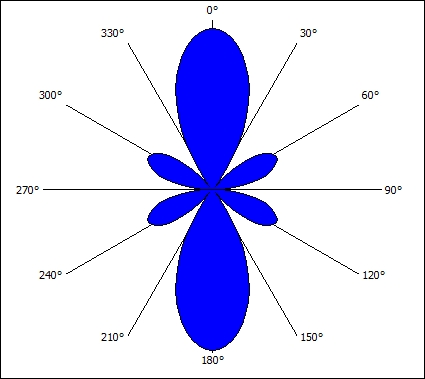
\includegraphics[width=\textwidth]{ressources/l3.jpg}\end{minipage}
        \caption[]%
        {{\small Theorie für $l=3$.}}
        \label{fig:2_12a}
    \end{subfigure}
    \hfill
    \begin{subfigure}[b]{0.475\textwidth}
        \centering
        \begin{minipage}{\textwidth}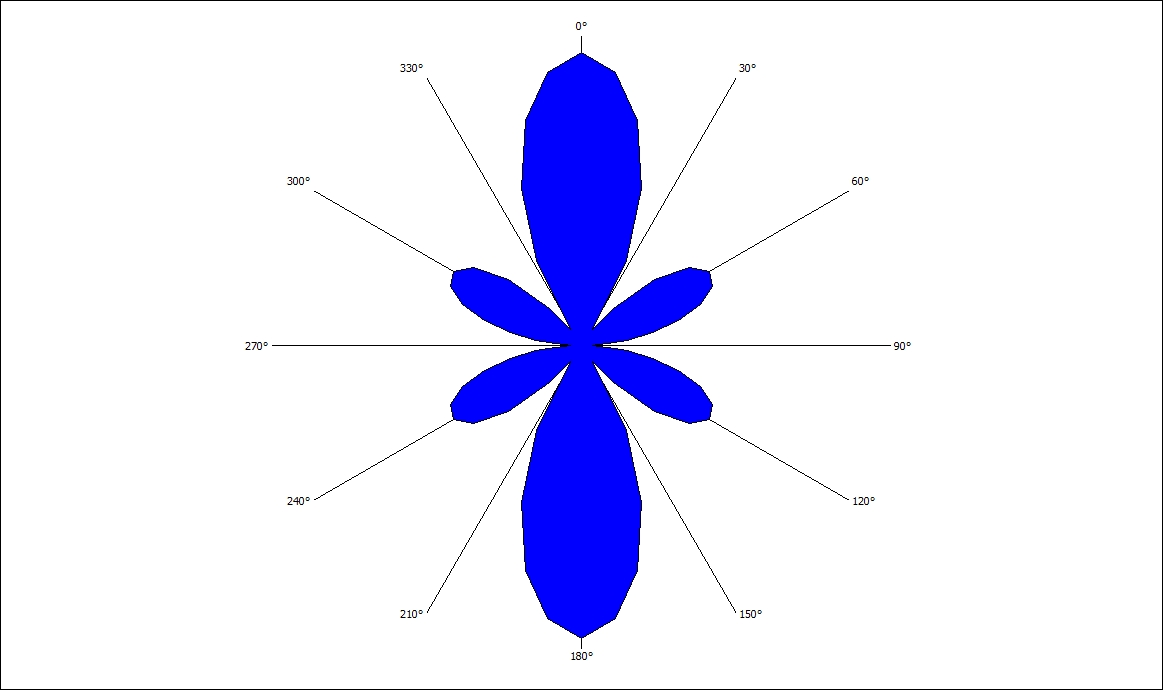
\includegraphics[width=\textwidth]{messdaten/2_3_4994.jpg}\end{minipage}
        \caption[]%
        {{\small Messung.}}
        \label{fig:2_12b}
    \end{subfigure}
    \caption[]
    {Polarplot für $f=\SI{4994}{\hertz}$.}
    \label{fig:2_12}
\end{figure}
\begin{figure}
    \centering
    \begin{subfigure}[b]{0.475\textwidth}
        \centering
        \begin{minipage}{\textwidth}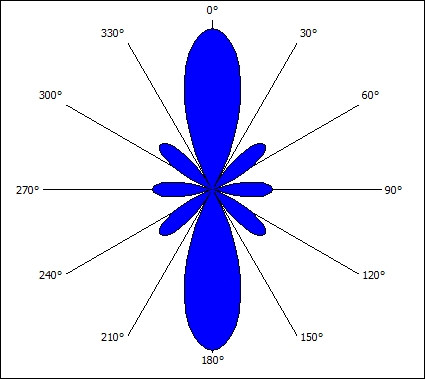
\includegraphics[width=\textwidth]{ressources/l4.jpg}\end{minipage}
        \caption[]%
        {{\small Theorie für $l=4$.}}
        \label{fig:2_13a}
    \end{subfigure}
    \hfill
    \begin{subfigure}[b]{0.475\textwidth}
        \centering
        \begin{minipage}{\textwidth}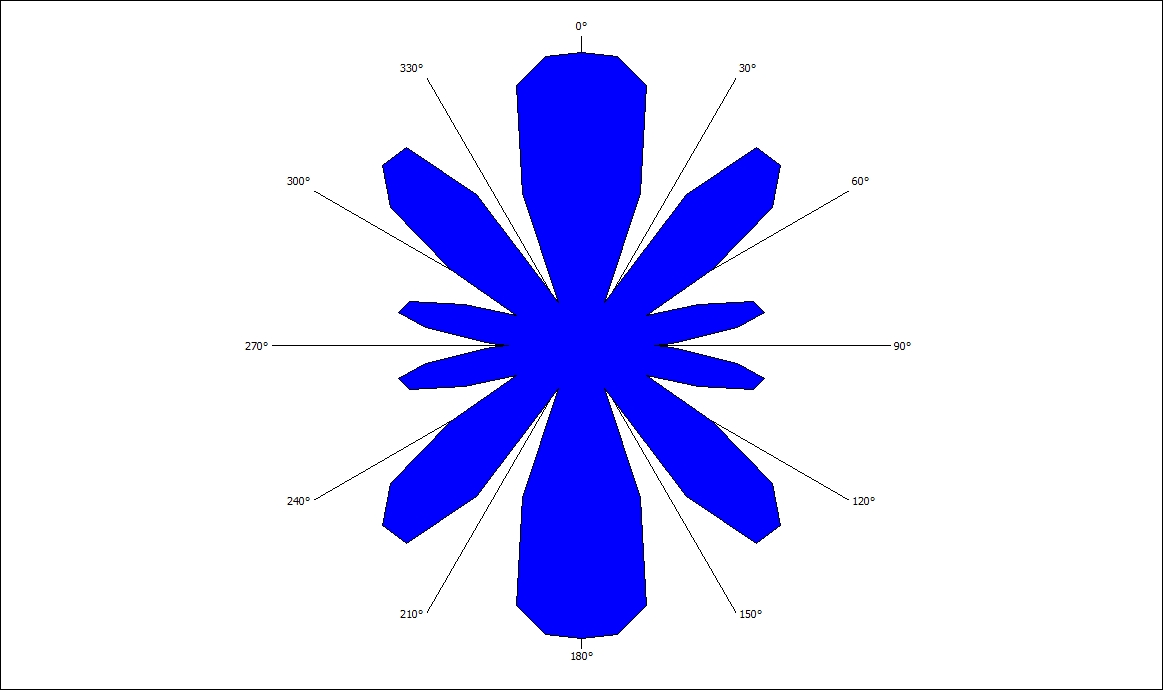
\includegraphics[width=\textwidth]{messdaten/2_3_6222.jpg}\end{minipage}
        \caption[]%
        {{\small Messung.}}
        \label{fig:2_13b}
    \end{subfigure}
    \caption[]
    {Polarplot für $f=\SI{6222}{\hertz}$.}
    \label{fig:2_13}
\end{figure}

\begin{figure}
  \centering
  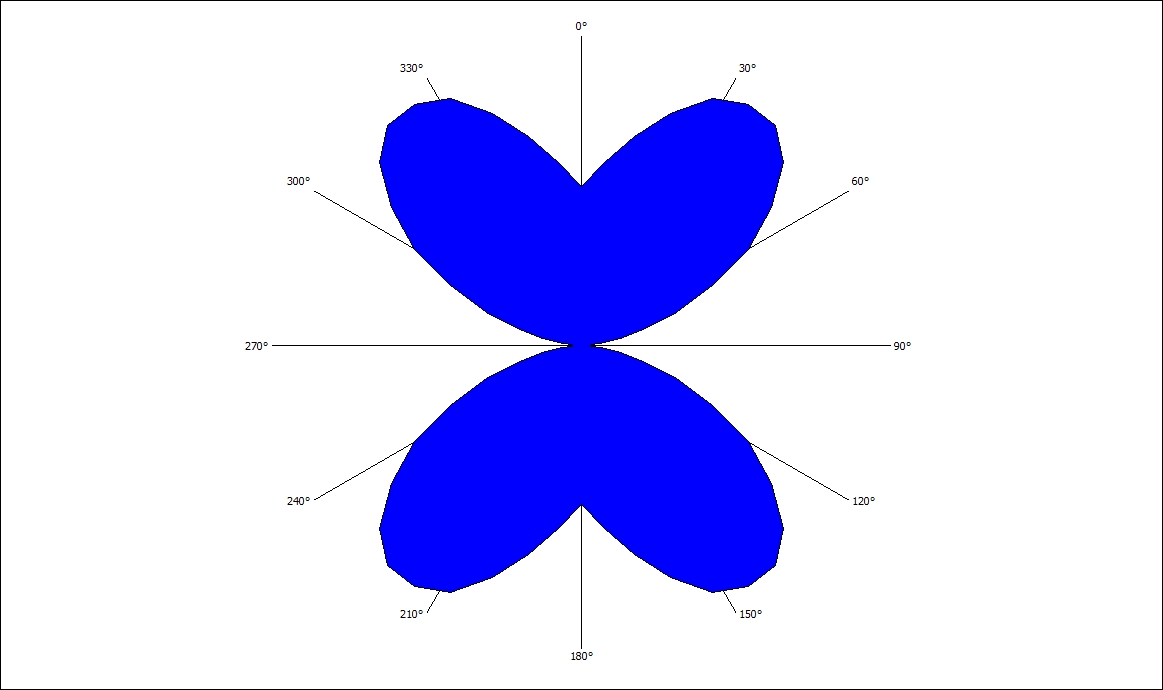
\includegraphics[width=0.45\textwidth]{messdaten/2_3_6572.jpg}  \caption{Polarplot für $f=\SI{6572}{\hertz}$. Eine Zuordnung für $l$ ist nicht möglich.} \label{fig:2_14}
\end{figure}
Die Zuordnung der Quantenzahl $l$ erfolgt anhand der Knotenzahl. Die Anzahl der Knoten in einer Hälfte des Polarplots ist gerade $l$, da die Quantenzahl $m$ aufgrund des Versuchsaufbau zu 0 gesetzt werden kann. Lediglich für den Peak um $f=\SI{6572}{\hertz}$ ist eine Zuordnung nicht möglich, denn der Polarplot weist keine Ähnlichkeit zu den Kugelflächenfunktionen auf. Somit wird die in Tabelle \ref{table:Zuordnung_l} angegebene Zuordnung getroffen.
\begin{table}
  \centering
  \caption{Zuordnung der Quantenzahl $l$.}
  \label{table:Zuordnung_l}
  \begin{tabular}{
% format 1.3 bedeutet eine Stelle vorm Komma, 3 danach
    S[table-format=1.0]
    S[table-format=1.0]
  }
    \toprule
    {$f \:/\: \si{\hertz}$} &
    {$l$} \\
    \midrule
    2310  &1 \\
    3711  &2 \\
    4994  &3 \\
    6222  &4 \\
    \bottomrule
  \end{tabular}
\end{table}
Es ist erkennbar, dass mit steigender Frequenz auch $l$ zunimmt. Dies ist ein experimentelles Indiz dafür, dass die Eigenwerte der Frequenz in der Helmholtz-Gleichung (siehe Gleichung \eqref{eq:Hemholtz}) eine Proportionalität zu $l$ aufweisen. Es wird im Übrigen darauf verzichtet, eine analytische Lösung von \eqref{eq:Hemholtz} anzugeben.

\subsection{Modellierung eines eindimensionalen Festkörpers}
\subsubsection{Bestimmung der Schallgeschwindigkeit}
\label{sec:Schallgeschwindigkeit}
Um die Schallgeschwindigkeit zu messen, werden stehende Schallwellen wie bereits in Kapitel \ref{sec:Ausw1} für verschiedene Längen aufgenommen. Die Ergebnisse sind in den Abbildungen \ref{fig:2_20} bis \ref{fig:2_27} zu sehen.
\begin{figure}
  \centering  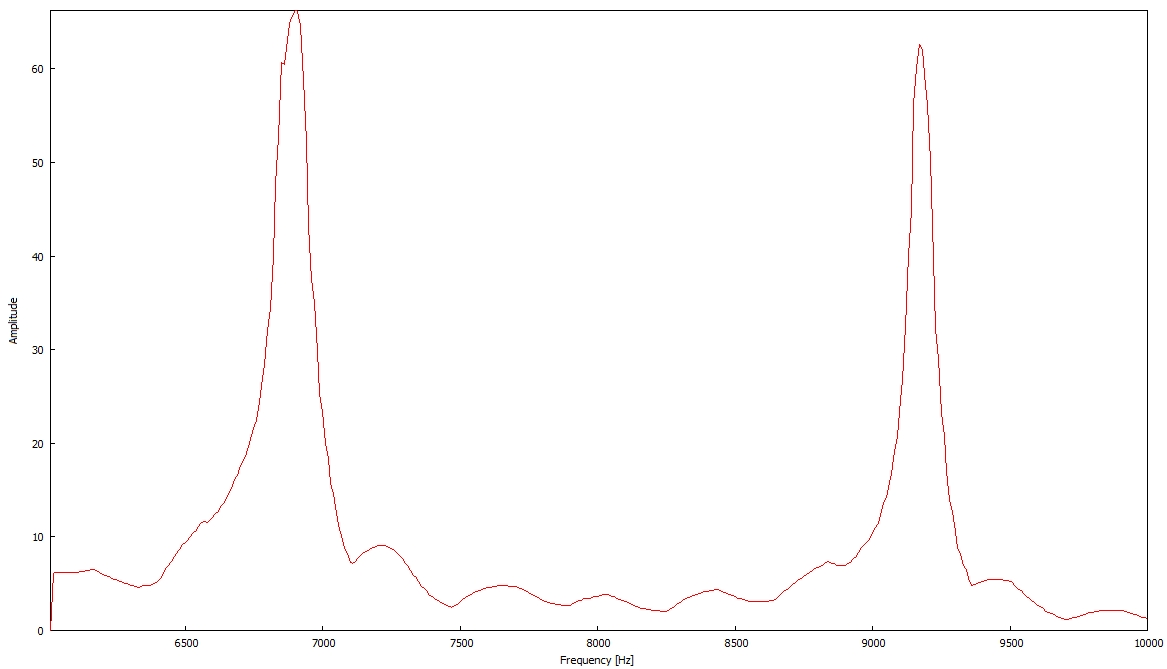
\includegraphics{build/3_1_75mm.pdf}  \caption{Messdaten einer 1$\times\SI{75}{\milli\meter}$ Röhre.} \label{fig:2_20}
\end{figure}
\begin{figure}
  \centering  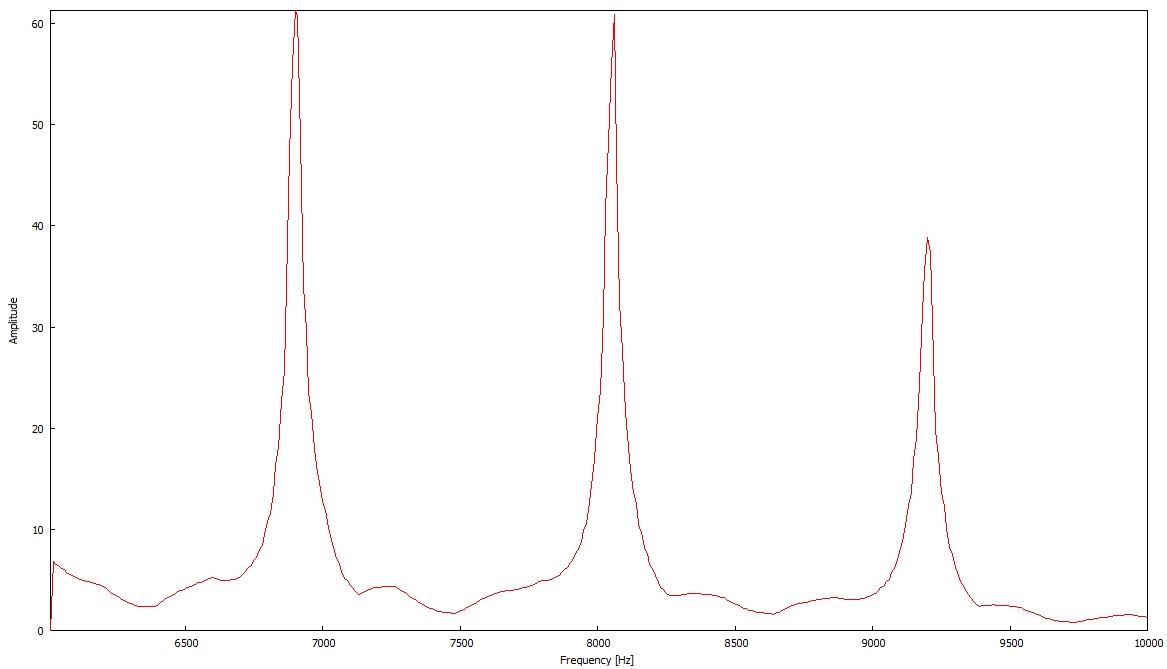
\includegraphics{build/3_1_150mm.pdf}  \caption{Messdaten einer 2$\times\SI{75}{\milli\meter}$ Röhre.} \label{fig:2_21}
\end{figure}
\begin{figure}
  \centering  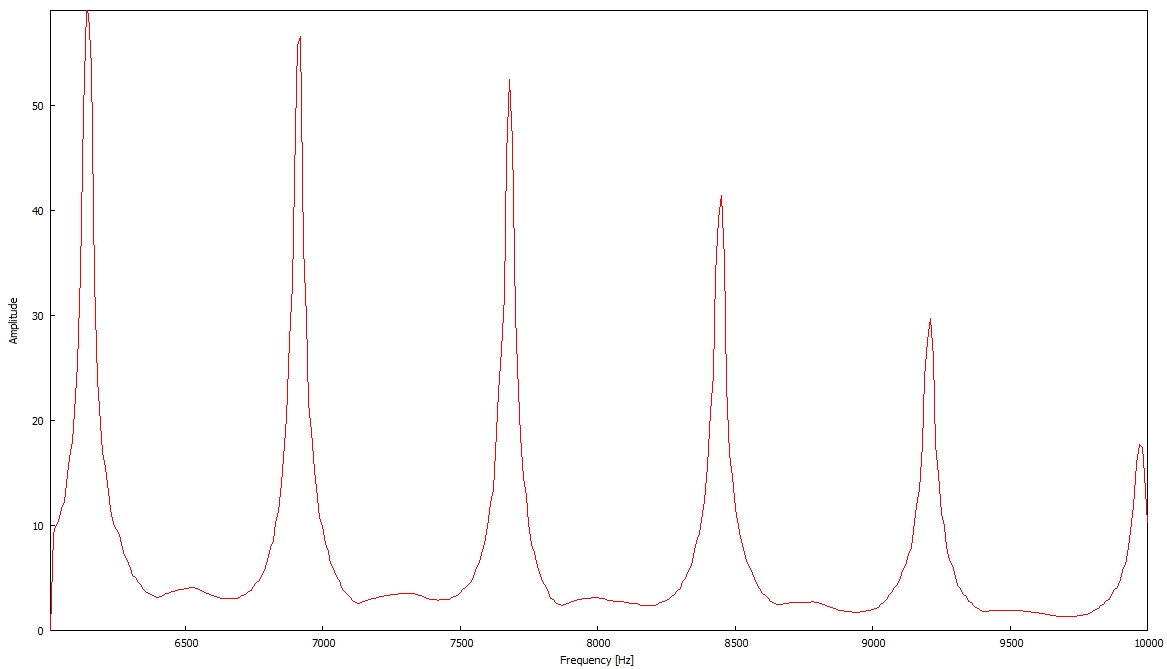
\includegraphics{build/3_1_225mm.pdf}  \caption{Messdaten einer 3$\times\SI{75}{\milli\meter}$ Röhre.} \label{fig:2_22}
\end{figure}
\begin{figure}
  \centering  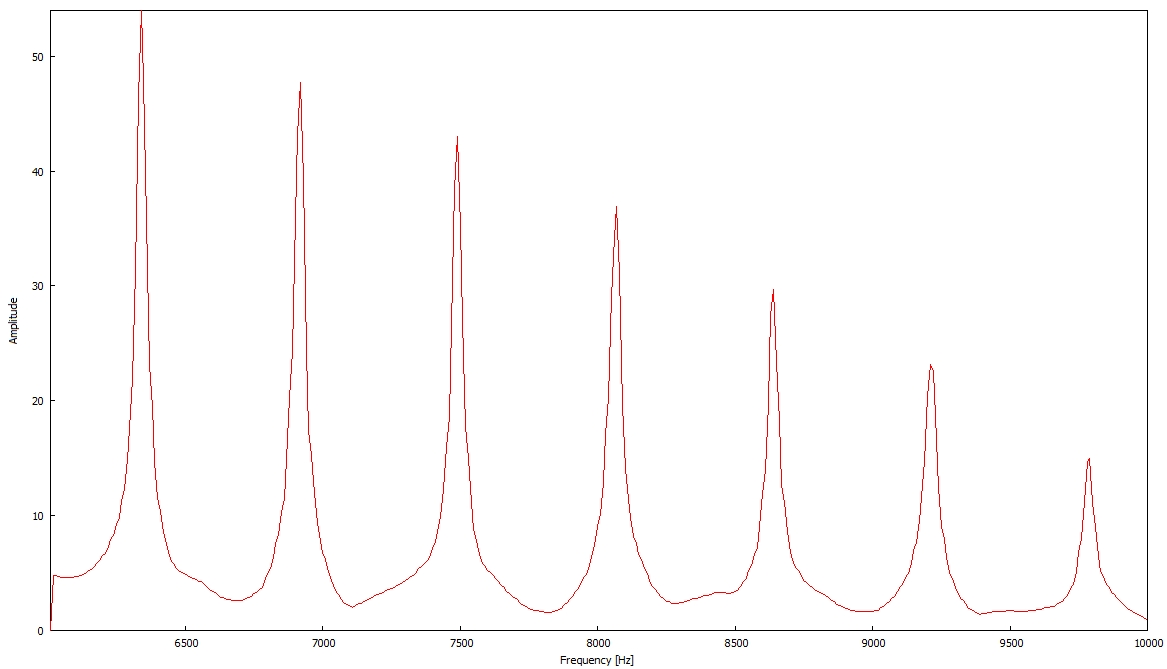
\includegraphics{build/3_1_300mm.pdf}  \caption{Messdaten einer 4$\times\SI{75}{\milli\meter}$ Röhre.} \label{fig:2_23}
\end{figure}
\begin{figure}
  \centering  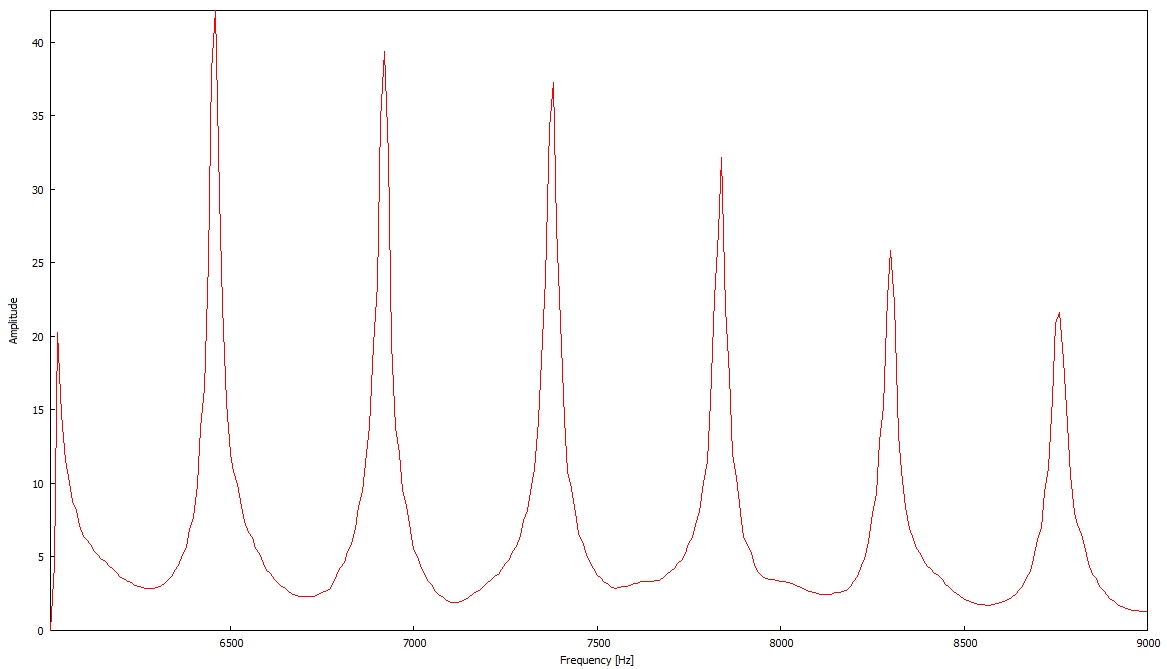
\includegraphics{build/3_1_375mm.pdf}  \caption{Messdaten einer 5$\times\SI{75}{\milli\meter}$ Röhre.} \label{fig:2_24}
\end{figure}
\begin{figure}
  \centering  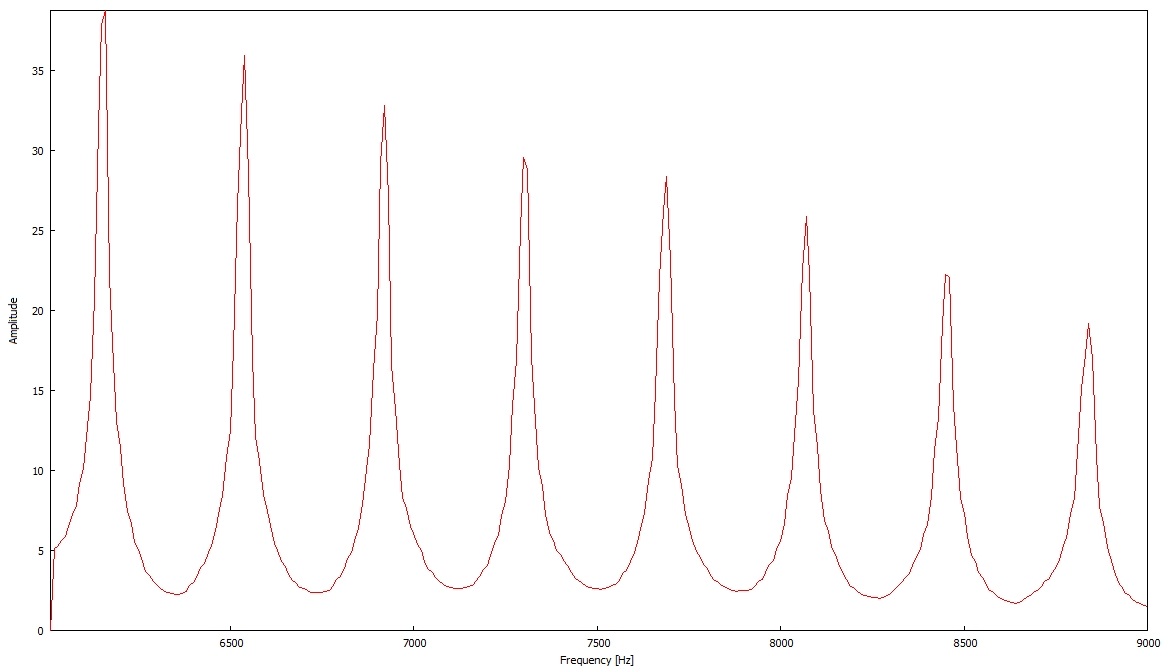
\includegraphics{build/3_1_450mm.pdf}  \caption{Messdaten einer 6$\times\SI{75}{\milli\meter}$ Röhre.} \label{fig:2_25}
\end{figure}
\begin{figure}
  \centering  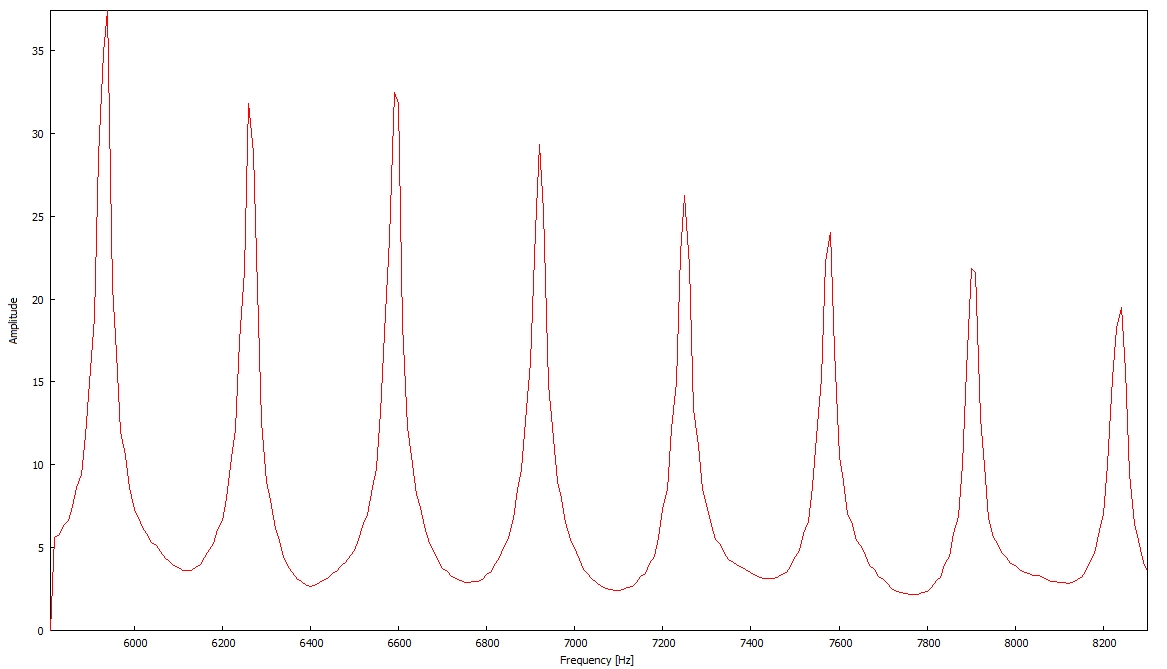
\includegraphics{build/3_1_525mm.pdf}  \caption{Messdaten einer 7$\times\SI{75}{\milli\meter}$ Röhre.} \label{fig:2_26}
\end{figure}
\begin{figure}
  \centering  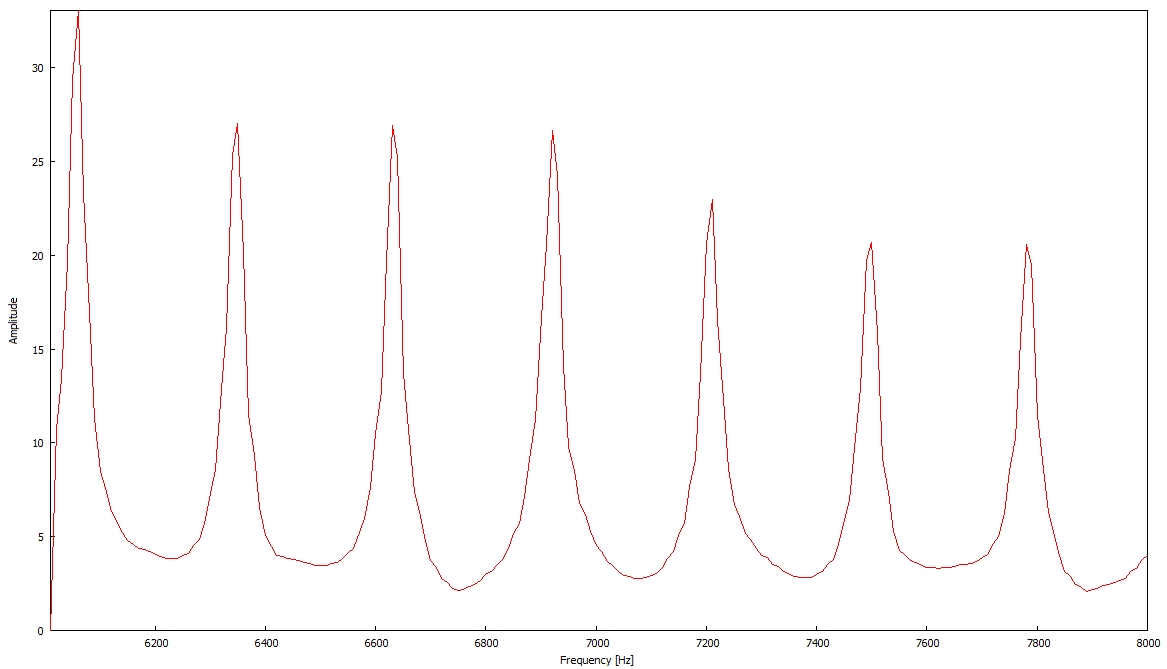
\includegraphics{build/3_1_600mm.pdf}  \caption{Messdaten einer 8$\times\SI{75}{\milli\meter}$ Röhre.} \label{fig:2_27}
\end{figure}
Von Interesse ist gemäß Gleichung \eqref{eq:Resonanz2} der Abstand zwischen zwei benachbarten Peaks. Um diese Abstände zu ermitteln, ist erneut das Herstellerprogramm SpectrumSLC verwendet worden. Die Spektren sind erneut mit der implementierten Fit-Funktion gefittet worden, um die Resonanzfrequenzen lokalisieren zu können. Die resultierenden Mittelwerte der Frequenz-Differenz zwischen zwei Peaks sind in Tabelle \ref{table:3_1_1} zusammen mit ihren Fehlern angegeben. Für die Länge $L=\SI{75}{\milli\meter}$ kann kein Fehler angegeben werden, da nur ein Messwert vorliegt und die Fitparameter aus der Software ohne Fehlerangaben gegeben sind.
\input{build/3_1_1.tex}
Nun wird eine lineare Regressionsrechnung in $1/L$ ausgeführt.
\begin{equation}
  \Delta f = a\frac{1}{L} + b
\end{equation}
Die gefundenen Parameter sind
\begin{align*}
  a &= \input{build/parameter_a.tex} \\
  b &= \input{build/parameter_b.tex} \; .
\end{align*}
Die Messwerte sind zusammen mit dem Fit in Abbildung \ref{fig:3_fitSchall} dargestellt.
\begin{figure}
  \centering  \includegraphics{build/3_fit.pdf}  \caption{Gemittelte Frequenzdifferenzen und linearer Fit.} \label{fig:3_fitSchall}
\end{figure}
Durch Vergleich mit Gleichung \eqref{eq:Resonanz2} ergibt sich die Schallgeschwindigkeit zu
\begin{align}
  c &= 2a = \input{build/Schallgeschwindigkeit.tex} .
  \label{eq:Schallgeschwindigkeit}
\end{align}
Im Vergleich mit dem Literaturwert bei 20°C \cite{sound}
\begin{equation*}
  c_\text{lit} = \SI{343.6}{\meter\per\second}
\end{equation*}
ergibt sich eine relative Abweichung von lediglich $\input{build/RelFehler_c.tex}$.

\subsubsection{Bestimmung der Wellenzahl}
Abbildung \ref{fig:3_20} zeigt das Übersichtsspektrum einer $\SI{60}{\centi\meter}$ langen Röhre.
\begin{figure}
  \centering  \includegraphics{build/3_20.pdf}  \caption{Spektrum einer 8$\times\SI{75}{\milli\meter}$ Röhre.} \label{fig:3_20}
\end{figure}
Außerdem eingezeichnet sind die mit einem open-source Paket für Python \cite{peakdetect} ermittelten Maxima der Amplitude. Diese werden nun mit $n$ durchnummeriert. Damit lässt sich die Wellenzahl gemäß
\begin{equation}
  k_n = n\frac{\pi}{L}
  \label{eq:k_von_n}
\end{equation}
berechnen. Die somit gefundenen Frequenzen und zugehörigen $k$-Werte sind in Tabelle \ref{table:3_2} zusammengestellt.
\input{build/3_2.tex}
Die hieraus abgeleitete Dispersionsrelation ist in Abbildung \ref{fig:3_21} zu sehen.
\begin{figure}
  \centering  \includegraphics{build/3_21.pdf}  \caption{Dispersionsrelation der 8$\times\SI{75}{\milli\meter}$ Röhre.} \label{fig:3_21}
\end{figure}
Da sowohl $f$ als auch $k$ linear mit n gehen, gilt theoretisch der lineare Zusammenhang
\begin{equation}
  f = \frac{c}{2\pi}k \; .
\end{equation}
Daher lässt sich hier erneut die Schallgeschwindigkeit aus einer linearen Regressionsrechnung in $k$ ermitteln. Der entsprechende Fit ist ebenfalls in Abbildung \ref{fig:3_21} eingezeichnet. Es ergeben sich die Fit-Parameter zu
\begin{align*}
  a &= \input{build/parameter_a2.tex} \\
  b &= \input{build/parameter_b2.tex} \; ,
\end{align*}
woraus die Schallgeschwindigkeit zu
\begin{align}
  c = 2\pi a = \input{build/Schallgeschwindigkeit2.tex}
\end{align}
folgt. Hier ist ein relativer Fehler von $\input{build/RelFehler_c2.tex}$ festzustellen. Dieser ist etwas größer als der in Kapitel \ref{sec:Schallgeschwindigkeit} gefundene Wert.

\subsubsection{Bandstruktur in einem periodischen Potential}
\label{sec:3.3}
Nun wird der eindimensionale Festkörper modelliert. Das Gitter des Festkörpers wird hierzu mit Blenden modelliert, welche periodische Streuzentren darstellen. Die Ergebnisse des ersten Versuchsteils (siehe Kapitel \ref{sec:Durchf3}) sind in den Abbildungen \ref{fig:3_30}, \ref{fig:3_31} und \ref{fig:3_32} zu sehen.
\begin{figure}
  \centering  \includegraphics{build/3_30_10mm.pdf}  \caption{Spektrum einer 8$\times\SI{50}{\milli\meter}$ Röhre mit $\SI{10}{\milli\meter}$ Iris.} \label{fig:3_30}
\end{figure}
\begin{figure}
  \centering  \includegraphics{build/3_30_13mm.pdf}  \caption{Spektrum einer 8$\times\SI{50}{\milli\meter}$ Röhre mit $\SI{13}{\milli\meter}$ Iris.} \label{fig:3_31}
\end{figure}
\begin{figure}
  \centering  \includegraphics{build/3_30_16mm.pdf}  \caption{Spektrum einer 8$\times\SI{50}{\milli\meter}$ Röhre mit $\SI{16}{\milli\meter}$ Iris.} \label{fig:3_32}
\end{figure}
Auch hier sind die Detektionen des Algorithmus \cite{peakdetect} eingezeichnet. Es ist zu beobachten, dass die Bänder mit zunehmender Frequenz schmaler werden. Ferner nimmt mit der Größe des Irisdurchmessers die Breite der Bänder zu und damit die Breite der Bandlücken ab. Dies ist klar, wenn zum Vergleich der Grenzfall einer nicht vorhandenen Iris herangezogen wird. Hierfür wird sich die periodische Struktur wie in Abbildung \ref{fig:3_20} einstellen. Dieser Grenzfall entspricht im Analogon einem freien Elektron. \\

Die gefundenen Frequenzen -- mit Ausnahme des 1. aufbaubedingten Peaks in Abbildung \ref{fig:3_30} -- werden in Tabelle \ref{table:Bandstruktur} zusammengefasst. Dabei sind dem ersten Band sieben $k$-Werte zugeordnet, denn die Resonanz für $k=0$ ist niemals sichtbar und es werden insgesamt pro Band genauso viele Peaks erwartet, wie Einheitszellen im Aufbau vorhanden sind, also acht. Die Frequenzen werden entsprechend in den nächsten achter-Block verschoben, falls sie sich im nächsten Band befinden. Die $k$-Werte werden erneut nach Gleichung \eqref{eq:k_von_n} berechnet.
\begin{table}
  \centering
  \caption{Messdaten und zugeordnete $n$- bzw. $k$-Werte.}
  \label{table:Bandstruktur}
  \sisetup{parse-numbers=false}
  \begin{tabular}{
% format 1.3 bedeutet eine Stelle vorm Komma, 3 danach
    S[table-format=2.0]
    S[table-format=5.0]
    S[table-format=5.0]
    S[table-format=5.0]
    S[table-format=5.0]
    S[table-format=3.1]
  }
    \toprule
    {$n$}
    & {$f_n(10\si{\milli\meter}) \:/\: \si{\hertz}$}
    & {$f_n(13\si{\milli\meter}) \:/\: \si{\hertz}$}
    & {$f_n(16\si{\milli\meter}) \:/\: \si{\hertz}$}
    & {$k_n \:/\: \si{\per\meter}$} \\
    \midrule
    \input{build/3_3_table_band1.tex}
    \midrule
    \input{build/3_3_table_band2.tex}
    \midrule
    \input{build/3_3_table_band3.tex}
    \midrule
    \input{build/3_3_table_band4.tex}
    \bottomrule
  \end{tabular}
\end{table}
Aus der Tatsache, dass die Bänder breiter mit zunehmendem Irisdurchmesser werden ergibt sich auch, dass die Auflösung der Peaks für größere Irisdurchmesser besser ist, was anhand der fehlenden Werte in der Tabelle für die beiden kleineren Durchmesser zu beobachten ist.
Die Daten in Tabelle \ref{table:Bandstruktur} bilden die Dispersionsrelation für das mechanische Analogon zum Elektron in einem Festkörper. Zur Visualisierung dient Abbildung \ref{fig:3_33}.
\begin{figure}
  \centering  \includegraphics{build/3_31.pdf}  \caption{Dispersionsrelation einer 8$\times\SI{50}{\milli\meter}$ Röhre mit verschiedenen Iris-Durchmessern.} \label{fig:3_33}
\end{figure}
Ferner erfolgt eine Abschätzung der Breite der Bänder $B_m$ (Tabelle \ref{table:bandbreiten}) und Bandlücken $G_m$ (Tabelle \ref{table:gapbreiten}). Die Werte werden in diesem Fall nicht durch eine Software, sondern "nach Augenmaß" anhand der Rohdaten bestimmt.
\begin{table}
  \centering
  \caption{Händisch gemessene Bandbreiten für versch. Iris-Durchmesser.}
  \label{table:bandbreiten}
  \sisetup{parse-numbers=false}
  \begin{tabular}{
    S[table-format=1.0]
    S[table-format=4.0]
    S[table-format=4.0]
    S[table-format=4.0]
  }
    \toprule
    {$m$}
    & {$B_m(10\si{\milli\meter}) \:/\: \si{\hertz}$}
    & {$B_m(13\si{\milli\meter}) \:/\: \si{\hertz}$}
    & {$B_m(16\si{\milli\meter}) \:/\: \si{\hertz}$}\\
    \midrule
    1 & 1720 & 2140 & 2430 \\
2 & 1020 & 1600 & 2120 \\
3 & 720  & 1130 & 1610 \\
4 & 600  & 960  & 1380 \\

    \bottomrule
  \end{tabular}
\end{table}
\begin{table}
  \centering
  \caption{Händisch gemessene Breiten der Bandlücken für versch. Iris-Durchmesser.}
  \label{table:gapbreiten}
  \sisetup{parse-numbers=false}
  \begin{tabular}{
    S[table-format=1.0]
    S[table-format=4.0]
    S[table-format=4.0]
    S[table-format=4.0]
  }
    \toprule
    {$m$}
    & {$G_m(10\si{\milli\meter}) \:/\: \si{\hertz}$}
    & {$G_m(13\si{\milli\meter}) \:/\: \si{\hertz}$}
    & {$G_m(16\si{\milli\meter}) \:/\: \si{\hertz}$}\\
    \midrule
    1 & 1500  & 930   & 670 \\
2 & 2380  & 1840  & 1290 \\
3 & 2670  & 2220  & 1700 \\

    \bottomrule
  \end{tabular}
\end{table}
Schließlich wird die Zustandsdichte gemäß der aus der Versuchsanleitung\cite{skript} entnommenen Gleichung
\begin{equation}
  \rho(f) = \frac{1}{f_{i+1}-f_i} \;\;\;\;\; (f_i\text{: Resonanzfrequenz})
\end{equation}
für den Aufbau mit einer $\SI{16}{\milli\meter}$ Iris berechnet und in Abbildung \ref{fig:Zustandsdichte} wiedergegeben. Die diskreten Punkte werden für einen besseren Eindruck in diesem Fall miteinander verbunden. In den Bandlücken wird die Zustandsdichte ferner auf 0 gesetzt -- hier sind Zustände per Definition nicht vorhanden.
\begin{figure}
  \centering  \includegraphics{build/3_32.pdf}  \caption{Zustandsdichte einer 8$\times\SI{50}{\milli\meter}$ Röhre mit verschiedenen Iris-Durchmessern.} \label{fig:Zustandsdichte}
\end{figure}
Gut zu erkennen sind die angedeuteten Van-Hove-Singularitäten an den Rändern der Bänder.

% 3.4
\subsubsection{Vergleich verschiedener Anzahlen von Einheitszellen}
\label{sec:3.4}
In diesem Teil werden drei Röhren, aufgebaut aus 8, 10 und 12 je $\SI{50}{\milli\meter}$ langen Röhren, miteinander verglichen. Es kommen Iriden mit $\SI{16}{\milli\meter}$ Durchmesser zum Einsatz. Die Spektren sind in den Abbildungen \ref{fig:3_32}, \ref{fig:3_40} und \ref{fig:3_41} zu sehen.
\begin{figure}
  \centering  \includegraphics{build/3_40.pdf}  \caption{Spektrum einer 10$\times\SI{50}{\milli\meter}$ Röhre mit $\SI{16}{\milli\meter}$ Iris.} \label{fig:3_40}
\end{figure}
\begin{figure}
  \centering  \includegraphics{build/3_41.pdf}  \caption{Spektrum einer 12$\times\SI{50}{\milli\meter}$ Röhre mit $\SI{16}{\milli\meter}$ Iris.} \label{fig:3_41}
\end{figure}
Wie zu erwarten nimmt die Anzahl der Maxima innerhalb eines Bandes erneut den Wert der Anzahl an Einheitszellen an, also jeweils 8, 10 und 12. Davon abgesehen sind die Spektren nahezu identisch, Bandbreiten und Breiten der Bandlücken sowie deren Position bleiben unverändert. Lediglich die Amplitudenwerte nehmen leicht ab mit steigender Röhrenlänge. Dies liegt an einer zunehmenden Dämpfung, bedingt durch die zusätzlichen Iriden.

% 3.5
\subsubsection{Vergleich verschiedener Einheitszellen}
Es verbleibt ein Vergleich zwischen Einheitszellen verschiedener Größe. Abbildung \ref{fig:3_50} zeigt hierzu das Spektrum einer Röhre mit acht je $\SI{75}{\milli\meter}$ langen Teilstücken und einer $\SI{16}{\milli\meter}$ Iris .
\begin{figure}
  \centering  \includegraphics{build/3_50.pdf}  \caption{Spektrum einer 8$\times\SI{75}{\milli\meter}$ Röhre mit $\SI{16}{\milli\meter}$ Iris.} \label{fig:3_50}
\end{figure}
Aufgrund der größeren Länge wird die Brillouin-Zone kleiner, wodurch mehr Brillouin-Zonen im selben Frequenz-Bereich sichtbar werden (sechs statt vier). Aus demselben Grund verschmalern sich die Bandlücken und Bänder. Nach wie vor wird ein Frequenzband durch acht Peaks gebildet, was ebenfalls den Erwartungen entspricht (siehe Kapitel \ref{sec:3.3}).

\subsection{Modellierung eines Atoms und Moleküls}
% # 3.6 und 3.7
\subsubsection{Einzelnes Atom}
\label{sec:3.6}
Das einzelne Atom wird durch eine einzelne Röhre simuliert. Abbildung \ref{fig:3_60} zeigt die Spektren einer $\SI{50}{\milli\meter}$ und einer $\SI{75}{\milli\meter}$ langen Röhre. Zusätzlich eingetragen sind die Peaks als Ergebnis des \emph{peakdetect} Algorithmus \cite{peakdetect}.
\begin{figure}
  \centering  \includegraphics{build/3_60.pdf}  \caption{Spektrum einer $\SI{75}{\milli\meter}$ und einer $\SI{50}{\milli\meter}$ Röhre mit detektierten Peaks.} \label{fig:3_60}
\end{figure}
Sichtbar sind lediglich longitudinale Moden. Radiale Moden sind aufgrund des Durchmessers der Röhre im Bereich von einem Zoll erst für höhere Frequenzen $f>\SI{16}{\kilo\hertz}$ zu erwarten. Die Soundkarte ist jedoch nicht in der Lage, diese zu detektieren, daher verschwindet das Signal ab ca. $\SI{13}{\kilo\hertz}$. Die Abstände zwischen zwei Resonanzen errechnen sich aus Gleichung \eqref{eq:Resonanz2} mit der Schallgeschwindigkeit aus Gleichung \eqref{eq:Schallgeschwindigkeit}. Dem gegenüber stehen die gemittelten Abstände aus der Messung, erneut mit dem \emph{peakdetect} Algorithmus ermittelt.
\begin{align*}
  \Delta f_{th,\text{50mm}} &= \input{build/3_6_delta_f50_th.tex}  & \Delta f_{exp,\text{50mm}} &= \SI{3405.0+-0.3}{\hertz}
\\
  \Delta f_{th,\text{75mm}} &= \input{build/3_6_delta_f75_th.tex}  & \Delta f_{exp,\text{75mm}} &= \input{build/3_6_delta_f75.tex}
\end{align*}
Hieraus ergibt sich eine relative Abweichung von $\input{build/3_6_relError50}$ für die $\SI{50}{\milli\meter}$ Röhre bzw. $\input{build/3_6_relError75}$ für die $\SI{75}{\milli\meter}$ Röhre. Der größere Fehler für $\Delta f_{exp,\text{75mm}}$ resultiert aus einer größeren Streuung der Frequenzdifferenzen für die $\SI{75}{\milli\meter}$ Röhre.

% 3.8
\subsubsection{Molekül aus zwei Atomen}
Nun werden zwei einzelne Atome zusammengebracht. Die Wechselwirkung zwischen ihnen wird durch eine Iris dargestellt. Der Durchmesser repräsentiert die Stärke der Wechselwirkung. Abbildung \ref{fig:3_80} zeigt die Spektren einer aus 2 je $\SI{50}{\milli\meter}$ langen Teilstücken aufgebauten Röhre mit verschiedenen Irisdurchmessern.
\begin{figure}
  \centering  \includegraphics{build/3_80.pdf}  \caption{Spektrum einer 2$\times\SI{50}{\milli\meter}$ Röhre für drei verschiedene Irisdurchmesser.} \label{fig:3_80}
\end{figure}
Zum Vergleich dient das auf den Frequenzbereich bis $\SI{12}{\kilo\hertz}$ zugeschnittene Spektrum einer einzelnen $\SI{50}{\milli\meter}$ langen Röhre in Abbildung \ref{fig:3_81}. Es ist zu erkennen, dass die einzelnen Resonanzen zu zwei Zuständen aufspalten. Dieser Effekt skaliert mit der Größe der Irisdurchmesser, dh. für die $\SI{16}{\milli\meter}$ Iris ist die Aufspaltung am größten. Die Zustände können dem bindendem (links in einem Band) und dem antibindendem (rechts in einem Band) Zustand zugeschrieben werden.
\begin{figure}
  \centering  \includegraphics{build/3_81.pdf}  \caption{Spektrum einer 1$\times\SI{50}{\milli\meter}$ Röhre.} \label{fig:3_81}
\end{figure}
% 3.9
\subsubsection{Molekül aus mehreren Atomen}
Nun wird die Anzahl an modellierten Atomen erhöht, das heißt es werden die Spektren mit 3, 4 und 6 Einheitszellen untersucht, siehe Abbildungen \ref{fig:3_90} bis \ref{fig:3_92}.
\begin{figure}
  \centering  \includegraphics{build/3_90.pdf}  \caption{Spektrum einer 3$\times\SI{50}{\milli\meter}$ Röhre für drei verschiedene Irisdurchmesser.} \label{fig:3_90}
\end{figure}
\begin{figure}
  \centering  \includegraphics{build/3_91.pdf}  \caption{Spektrum einer 4$\times\SI{50}{\milli\meter}$ Röhre für drei verschiedene Irisdurchmesser.} \label{fig:3_91}
\end{figure}
\begin{figure}
  \centering  \includegraphics{build/3_92.pdf}  \caption{Spektrum einer 6$\times\SI{50}{\milli\meter}$ Röhre für drei verschiedene Irisdurchmesser.} \label{fig:3_92}
\end{figure}
Die Beobachtungen sind analog zu denen aus Kapitel \ref{sec:3.4}. Die Bänder spalten sich immer weiter auf. Im Grenzwert unendlich vieler Einheitszellen sind kontinuierliche Bänder zu erwarten mit den bereits gefundenen Bandlücken dazwischen.

% 3.10
\subsubsection{Superstruktur, alternierende Iriden}
In Abbildung \ref{fig:3_100} ist das Spektrum einer Superstruktur bestehend aus den zwei alternierend aufgestellten Einheitszellen. Die Einheitszellen werden aus einer $\SI{50}{\milli\meter}$ Röhre, gefolgt von einer $\SI{13}{\milli\meter}$ Iris (Einheitszelle 1) bzw. einer $\SI{16}{\milli\meter}$ Iris (Einheitszelle 2) aufgebaut. Insgesamt kommt jede Einheitszelle vier mal vor. Zum Vergleich ist auch das Spektrum aus Abbildung \ref{fig:3_41} eingezeichnet. Dabei handelt es sich um eine Anordnung aus 8$\times\SI{50}{\milli\meter}$ Stücken, getrennt durch $\SI{16}{\milli\meter}$ Iriden.
\begin{figure}
  \centering  \includegraphics{build/3_100.pdf}  \caption{Spektrum der Superstruktur (siehe Text).} \label{fig:3_100}
\end{figure}
Zu Beobachten ist, dass die Bänder im Fall der Superstruktur schmaler werden, aber innerhalb der Bänder der ungestörten Struktur liegen. Dies ist vermutlich auf die kleineren Irisdurchmesser der Einheitszelle 1 zurückzuführen, welche effektiv wie bereits in Kapitel \ref{sec:3.3} diskutiert zu einer Verschmalerung der Bänder führen. Ferner ist festzuhalten, dass ungefähr in der Mitte eines Bandes eine kleine Bandlücke entstanden ist. Dies ist eine Folge der verwendeten Superstruktur.
In Abbildung \ref{fig:3_101} ist die Dispersionsrelation zu sehen. Sie ergibt sich nach dem Verfahren aus Kapitel \ref{sec:3.3}, allerdings wird diesmal darauf verzichtet, die Anzahl der Peaks auf die eigentlich vorhandenen künstlich zu erweitern. Werden also in einem Band wenige Frequenzmaxima detektiert, so verschieben sich die weiteren Zuordnungen zu kleinere $k$-Werten. Trotzdem ist die Struktur, wie beispielsweise die Bandlücken, gut zu erkennen.
\begin{figure}
  \centering  \includegraphics{build/3_101.pdf}  \caption{Dispersionsrelation der Superstruktur sowie der Referenz.} \label{fig:3_101}
\end{figure}

% 3.11
\subsubsection{Superstruktur, alternierende Teilstücklängen}
In diesem Versuchsteil werden zwei unterschiedliche Einheitszellen alternierend angeordnet. Eine Einheitszelle besteht aus einem $\SI{50}{\milli\meter}$ Stück mit einer $\SI{16}{\milli\meter}$ Iris, die andere aus einem $\SI{75}{\milli\meter}$ Stück ebenfalls mit einer $\SI{16}{\milli\meter}$ Iris. Das Spektrum ist in Abbildung \ref{fig:3_110} zu sehen.
\begin{figure}
  \centering  \includegraphics{build/3_110.pdf}  \caption{Spektrum der Superstruktur (siehe Text).} \label{fig:3_110}
\end{figure}
Zum Vergleich sind auch die Spektren einzelner Teilstücke aus Kapitel \ref{sec:3.6} eingezeichnet. In dem Spektrum Superstruktur ist zu erkennen, dass zwei einzelne Frequenzbänder periodisch wiederkehren, in ihrer Amplitude jedoch mit der Frequenz abnehmen. Es ist zu erwarten, dass diese Bänder jeweils die Aufspaltungen der Resonanzen der beiden einzelnen Einheitszellen sind, jedoch ist diese Erwartung anhand der Grafik nur schwierig zu verifizieren, denn beispielsweise fällt der Peak des blau eingezeichneten Spektrums um $\SI{3.5}{\kilo\hertz}$ im Superspektrum in eine Bandlücke. Andererseits ist aufgrund der geänderten Gesamtlänge des Aufbaus eine "Verdichtung" der Einzelspektren zu erwarten, das heißt dass die Resonanzen weiter zusammen rücken. % DISKUSSION - Erklärung is real
Abbildung \ref{fig:3_111} zeigt die Dispersionsrelation der Superstruktur mit alternierenden Teilstücklängen. Dabei ist erneut wie im letzten Abschnitt vorgegangen worden.
\begin{figure}
  \centering  \includegraphics{build/3_111.pdf}  \caption{Dispersionsrelation der Superstruktur mit alternierenden Teilstücklängen.} \label{fig:3_111}
\end{figure}

% 3.12
\subsubsection{Defekte}
Im Folgenden wird der Einfluss eines Defektes in einer ansonsten regelmäßigen Struktur (ohne Superstruktur) untersucht. Abbildung \ref{fig:3_120} zeigt hierzu die Spektren einer 12$\times\SI{50}{\milli\meter}$ Röhre mit $\SI{16}{\milli\meter}$ Iriden und einer Konfiguration, wo an Position 3 in der Kette ein $\SI{50}{\milli\meter}$ Stück durch ein $\SI{75}{\milli\meter}$ Stückt ersetzt ist.
\begin{figure}
  \centering  \includegraphics{build/3_120.pdf}  \caption{Einfluss eines eingebauten Defekts auf das Spektrum.} \label{fig:3_120}
\end{figure}
Hierfür wird gemäß dem Vorgehen aus den letzten beiden Abschnitten die Dispersionsrelation erstellt, siehe Abbildung \ref{fig:3_121}.
\begin{figure}
  \centering  \includegraphics{build/3_121.pdf}  \caption{Einfluss eines eingebauten Defekts auf die Dispersionsrelation.} \label{fig:3_121}
\end{figure}
Erwartungsgemäß ist der Einfluss des Defektes auf das Spektrum und somit die Dispersionsrelation nicht groß. Die ursprüngliche Bandstruktur wird weitestgehend beibehalten, jedoch wird ein Zustand innerhalb einer Bandlücke bei ca. $\SI{3}{\kilo\hertz}$ beobachtet. Auch bei ca. $\SI{5.3}{\kilo\hertz}$ gibt es einen kaum erkennbaren solchen Ausreißer. Damit ist die Anzahl Maxima tatsächlich erhalten, wobei ein Zustand in der Bandlücke liegt, und dafür im Band selbst einer weniger zu finden ist. Es sind nach wie vor zwölf Peaks. Hier ist schön zu sehen, dass durch einen Defekt Zustände in der Bandlücke eingebaut werden, genauso wie es auch beim Dotieren von Halbleitern geschieht.\\
Abschließend wird der Einfluss der Position sowie der Größe des Defekts untersucht. Abbildung \ref{fig:3_122} zeigt hierzu das Spektrum für denselben Defekt an verschiedenen Positionen, während Abbildung \ref{fig:3_123} den Einfluss der Defektgröße zum Vorschein bringt.
\begin{figure}
  \centering  \includegraphics{build/3_122.pdf}  \caption{Einfluss der Position des eingebauten Defekts bei gleicher Größe $L_D=\SI{75}{\milli\meter}$ des Defekts.} \label{fig:3_122}
\end{figure}
\begin{figure}
  \centering  \includegraphics{build/3_123.pdf}  \caption{Einfluss der Größe des eingebauten Defekts bei gleichbleibender Position 3 des Defekts.} \label{fig:3_123}
\end{figure}
Auffällig ist in Abbildung \ref{fig:3_123}, dass das erste Band für $L_D=\SI{12.5}{\milli\meter}$ lediglich 10 Peaks statt den erwarteten 11 enthält. In diesem Vergleich ist ferner eine Verschiebung der Maxima zu verzeichnen, nicht jedoch der Bänder oder Bandlücken an sich. Der Defektzustand bei ca. $\SI{3}{\kilo\hertz}$ verschiebt sich ebenfalls. Da die Anzahl der Peaks gleich bleibt, diese jedoch untereinander verschoben sind, ist klar, dass die ursprüngliche Periodizität aufgehoben ist. Ein Mittelwert von $\Delta f$ hätte nun eine deutlich größere Varianz. Die Wellenzahl kann daher auch nicht mehr als "gute Quantenzahl" angesehen werden. \\
Beim Vergleich verschiedener Positionen in Abbildung \ref{fig:3_122} ist zu sehen, dass das erste Band kaum betroffen ist, während das zweite Band sowohl Verschiebungen der Maxima als auch starke Variationen in der Amplitudenhöhe aufweist. Der Defektzustand in der Energielücke ist insbesondere für Position 1 deutlich weiter links. Eine exakte Begründung für diesen Sachverhalt verbleibt ausstehend. Allerdings lässt sich hieran erkennen, dass das Experiment aufgrund der endlichen Länge L nicht ein periodisches Gitter modellieren kann. In diesem wäre die Position der Fehlstelle irrelevant.


% Sämtliche im Folgenden durchgeführten Ausgleichsrechnungen werden mit der \emph{curve fit} Funktion aus dem für \emph{Python} geschriebenen package \emph{NumPy}\cite{scipy} durchgeführt. Fehlerrechnungen werden mit dem für \emph{Python} geschriebenen package \emph{Uncertainties}\cite{uncertainties} ausgeführt.

% % Examples
% \begin{equation}
%   U(t) = a \sin(b t + c) + d
% \end{equation}
%
% \begin{align}
%   a &= \input{build/a.tex} \\
%   b &= \input{build/b.tex} \\
%   c &= \input{build/c.tex} \\
%   d &= \input{build/d.tex} .
% \end{align}
% Die Messdaten und das Ergebnis des Fits sind in Abbildung~\ref{fig:plot} geplottet.
%
% %Tabelle mit Messdaten
% \begin{table}
%   \centering
%   \caption{Messdaten.}
%   \label{tab:data}
%   \sisetup{parse-numbers=false}
%   \begin{tabular}{
% % format 1.3 bedeutet eine Stelle vorm Komma, 3 danach
%     S[table-format=1.3]
%     S[table-format=-1.2]
%     @{${}\pm{}$}
%     S[table-format=1.2]
%     @{\hspace*{3em}\hspace*{\tabcolsep}}
%     S[table-format=1.3]
%     S[table-format=-1.2]
%     @{${}\pm{}$}
%     S[table-format=1.2]
%   }
%     \toprule
%     {$t \:/\: \si{\milli\second}$} & \multicolumn{2}{c}{$U \:/\: \si{\kilo\volt}$\hspace*{3em}} &
%     {$t \:/\: \si{\milli\second}$} & \multicolumn{2}{c}{$U \:/\: \si{\kilo\volt}$} \\
%     \midrule
%     1.7 & 10 \\
2.3 & 20 \\
3.5 & 30 \\
4.4 & 40 \\

%     \bottomrule
%   \end{tabular}
% \end{table}
%
% % Standard Plot
% \begin{figure}
%   \centering
%   \includegraphics{build/plot.pdf}
%   \caption{Messdaten und Fitergebnis.}
%   \label{fig:plot}
% \end{figure}
%
% 2x2 Plot
% \begin{figure*}
%     \centering
%     \begin{subfigure}[b]{0.475\textwidth}
%         \centering
%         \includegraphics[width=\textwidth]{Abbildungen/Schaltung1.pdf}
%         \caption[]%
%         {{\small Schaltung 1.}}
%         \label{fig:Schaltung1}
%     \end{subfigure}
%     \hfill
%     \begin{subfigure}[b]{0.475\textwidth}
%         \centering
%         \includegraphics[width=\textwidth]{Abbildungen/Schaltung2.pdf}
%         \caption[]%
%         {{\small Schaltung 2.}}
%         \label{fig:Schaltung2}
%     \end{subfigure}
%     \vskip\baselineskip
%     \begin{subfigure}[b]{0.475\textwidth}
%         \centering
%         \includegraphics[width=\textwidth]{Abbildungen/Schaltung4.pdf}    % Zahlen vertauscht ... -.-
%         \caption[]%
%         {{\small Schaltung 3.}}
%         \label{fig:Schaltung3}
%     \end{subfigure}
%     \quad
%     \begin{subfigure}[b]{0.475\textwidth}
%         \centering
%         \includegraphics[width=\textwidth]{Abbildungen/Schaltung3.pdf}
%         \caption[]%
%         {{\small Schaltung 4.}}
%         \label{fig:Schaltung4}
%     \end{subfigure}
%     \caption[]
%     {Ersatzschaltbilder der verschiedenen Teilaufgaben.}
%     \label{fig:Schaltungen}
% \end{figure*}
